\section{An Infrastructure for Non-functional Testing Using System Containers}
In general, there are many non-functional properties that can be influenced by compiler optimizations, \eg, performance (execution time), code quality, robustness, etc. In this paper, we focus on the efficiency of optimized code in term of resource consumption (memory and CPU).
Therefore, we need to deploy the test harness, i.e., the produced binaries, on an elastic infrastructure that provides to compiler users facilities to ensure the deployment and monitoring of different variants of optimized code. 
%Monitoring information should also be provided to inform about resource utilization required/needed and to automate the resource management of deployed components. 
For this purpose, we propose NOTICE, a non-functional testing infrastructure based on System Container techniques such as Docker\footnote{\url{https://www.docker.com}} environment. 

%Docker will automate the deployment and execution of applications inside software containers by allowing multiple applications to run autonomously on a server (basically a cloud server). 
%It provides a platform as a service (PaaS) style of deployment for software programs. 
Consequently, we rely on this technology and benefit from all its advantages to:
\begin{enumerate}
	\item Deploy generated code within containers
	\item Automate optimization sequences generation
	\item Execute and monitor service containers
	\item Gather performance metrics (CPU, Memory, I/O, etc.)
\end{enumerate}

%We integrate a collection of containers to define the adequate infrastructure for testing and monitoring of compilers. 

Before starting to monitor and test generated code, we have to describe the deployment environment of NOTICE.
\subsection{System Containers as Deployment Environment}

NOTICE represents a component-based infrastructure based on Docker Linux containers to monitor the execution of produced binaries by compilers in term of resource usage. 
Docker is an open source engine that automates the deployment of any application as a lightweight, portable, and self-sufficient container that runs virtually on a host machine. 
%To achieve that, Docker uses the Linux container technology. 
Using Docker, we can define preconfigured applications and servers to host as virtual images. We can also define the way the service should be deployed in the host machine. 
%As properties, we can define the OS where the service has to run, dependencies, etc. 
A simple way to build images automatically is to use Dockerfiles which represents configuration files.
%Docker can build images automatically by reading the instructions from a Dockerfile. 
We use Docker Hub\footnote{https://hub.docker.com/} for building, saving, and managing all our Docker images. It represents a cloud-based registry service for building and shipping application or service containers.
Once Docker images are defined, we can instantiate different containers. 
%Basically, each container deploys an optimized version of the input source code program.

Therefore, to run our experiments, each optimized program is executed individually inside an isolated Linux container. By doing so, we ensure that each executed program runs in isolation without being affected by the host machine or any other processes. Moreover, since a container is cheap to create, we are able to create too many containers as long as we have new programs to execute. 
Since each program execution requires a new container to be created, it is crucial to remove and kill containers that have finished their job to eliminate the load on the system. In fact, containers/programs are running sequentially without defining any resource constraints. So once execution is done, resources reserved for the container are automatically released to enable spawning next containers. Therefore, the host machine will not suffer too much from the performance trade-offs.

We resume, in the following, the main advantages of this approach:
\begin{enumerate}
	\item The use of containers induces less performance overhead and resource isolation compared to using a full stack virtualization solution. Instrumentation tools for memory profiling like Valgrind~\cite{nethercote2007valgrind} can induce too much overhead.
	\item Thanks to the use of Dockerfile, NOTICE can be easily configured by compiler users to define the target compiler to test (\eg, GCC compiler version), the container OS, the input program under test and the optimization options, etc. Thus, NOTICE uses the same configured Docker image to execute different instances of generated code. For hardware architecture, containers share the same platform architecture as the host machine (e.g., x86, x64, ARM, etc.). 
	\item Docker uses Linux control groups (cgroups) to group processes running in the container. This allows us to manage the resources of a group of processes, which is very valuable. 
	This approach increases the flexibility when we want to manage resources, since we can manage every group individually. 
	\item Although containers run in isolation, they can share data with the host machine and other running containers. Thus, non-functional data relative to resource consumption can be easily gathered and managed by other containers (i.e., for storage purpose, visualization)
\end{enumerate}


\subsection{Runtime Testing Components}
In order to test our running applications within Docker containers, we aim to use a set of Docker components to ease the extraction of non-functional properties related to resource usage.
\subsubsection{Monitoring Component}
This container will provide us an understanding of the resource usage and performance characteristics of our running containers. Generally, Docker containers rely on cgroups file systems to expose a lot of metrics about accumulated CPU cycles, memory, block I/O usage, etc. Therefore, our monitoring component automates the extraction of runtime performance metrics using cgroups. For example, we access to live resource consumption of each container available at the cgroup file system via stats found in $/sys/fs/cgroup/cpu/docker/(longid)/$ (for CPU consumption) and $/sys/fs/cgroup/memory/docker/(longid)/$ (for stats related to memory consumption). This component will automate the process of service discovery and metrics aggregation. Thus, instead of gathering manually metrics located in cgroups file systems, it will extract automatically runtime resource usage statistics relative to running components. We note that resource usage information is collected in raw data. This process may induce a little overhead, because it does very fine-grained accounting of resource usage on running container. Fortunately, this may not affect the gathered performance values since NOTICE run only one optimized version of code within each container.

To ease the monitoring process, NOTICE integrates google containers called cAdvisor as Container Advisor\footnote{https://github.com/google/cadvisor}. It is a tool developed by Google to monitor their infrastructure. 
cAdvisor Docker image does not need any configuration on the host machine. We have just to run it on our host machine. It will then have access to resource usage and performance characteristics of all running containers. This image uses the cgroups mechanism described above to collect, aggregate, process, and export ephemeral real-time information about running containers. Then, it reports all statistics via web UI ($http://localhost:8080$) to view live resource consumption of each container. cAdvisor has been widely used in different projects such as Heapster\footnote{https://github.com/kubernetes/heapster} and Google Cloud Platform\footnote{https://cloud.google.com/}.

However, cAdvisor monitors and aggregates live data over only 60 seconds interval. Therefore, we would like to record all data over time since container's creation. This is useful to run queries and define non-functional metrics from historical data. Thereby, to make gathered data truly valuable for resource usage monitoring, it becomes necessary to log it into a database at runtime. Thus, we link our monitoring component to a back-end database. 
\subsubsection{Back-end Database Component}
This component represents a times-series database back-end. It is plugged with the previously described monitoring component to save the non-functional data for long-term retention, analytics and visualization. Hence, we define its corresponding ip port into the monitoring component so that, container statistics are sent over TCP port (e.g., 8083) exposed by the database component.

During the execution of generated code, resource usage stats are continuously sent to this component. When a container is killed, NOTICE is able to access to its relative resource usage metrics through the database. We choose a time series database because we are collecting time series data that corresponds to the resource utilization profiles of programs execution.

We use InfluxDB\footnote{https://github.com/influxdata/influxdb}, an open source distributed time series database as a back-end to record data. InfluxDB allows the user to execute SQL-like queries on the database. For example the following query reports the maximum memory usage of container $"generated\_code\_v1"$ since its creation:

\begin{lstlisting}[
language=SQL,
showspaces=false,
basicstyle=\small,
numberstyle=\small,
commentstyle=\color{gray},
linewidth=\columnwidth
]
select max (memory_usage) from stats 
where container_name='generated_code_v1'
\end{lstlisting}
To give an idea about data stored in InfluxDB, Table 1 describes the different stored metrics:
 \begin{table}[h]
 	\begin{center}
 		\begin{tabular}{|p{1cm}|p{6.9cm}|}
 			\hline
 			 \textbf{Metric} & \textbf{Description} \\
 		\hhline{|=|=|}	
 			 Name & Container Name \\
 		
 			 T & Elapsed time since container's creation \\
 		
 			 Network &  Stats for network bytes and packets in an out of the container \\
 		
 			 Disk IO &  Disk I/O stats \\
 		
 			 Memory &  Memory usage \\
 			
 		   	 CPU &  CPU usage \\
 			\hline
 			
 		\end{tabular}
 		
 	\end{center}
 	\caption {Resource usage metrics recorded in InfluxDB}
 	%\vspace*{-0.9cm}
 \end{table}
 
Apart from that, NOTICE provides also information about the size of generated binaries and the compilation time needed to produced code.
For instance, resource usage statistics are collected and stored using NOTICE. It would be nice to view resource consumption graphs within a complete dashboard. It is relevant to show performance profiles of memory and CPU consumption of our running programs overtime. To do so, we present a front-end visualization component for performance profiling. 

\subsubsection{Front-end Visualization Component}
%Once we gather and store resource usage data, the next step is visualizing them. That is the role of the visualization component. It will be the endpoint component that we use to visualize the recorded data. 
NOTICE provides a dashboard to run queries and view different profiles of resource consumption of running components through web UI. 
Thanks to this component, we can compare visually the profiles of resource consumption of running containers. 
%Moreover, we use this component to export the data currently being viewed into static CSV document. 
%Thereby, we can perform statistical analysis and process data to analyze performance behavior. 
%An overview of the monitoring dashboard is shown in Figure 3.

To do so, we choose Grafana\footnote{https://github.com/grafana/grafana}, one of the best time-series visualization tools available for Docker. It is considered as a web application running within a container. We run Grafana and we link it to InfluxDB by setting up the data source port 8086 so that, it can easily request data from the database. 
We recall that InfluxDB also provides a web UI to query the database and show graphs. But, Grafana will let us to display live results over time in much pretty looking graphs. Same as InfluxDB, we use SQL queries to extract non-functional metrics from the database for visualization.

\subsection{Wrapping Everything Together: Architecture Overview}
To summarize, we present, in Figure 3, an overall overview of the different components involved within NOTICE.

\begin{figure}[h]
\centering
	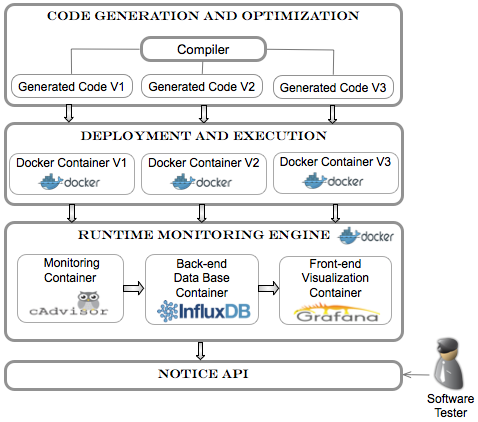
\includegraphics[width=1.\linewidth]{Ressources/genecoApproach.png}
	\caption{NOTICE architecture overview}
\end{figure}


Our testing infrastructure will run different jobs within Docker containers. First, in the top level layer, we use NOTICE to generate different versions of code using our target compiler (e.g., GCC compiler). Then, we wrap generated code within multiple instances of our preconfigured Docker image. Each container will execute a specific job. For our case, a job represents a program compiled with a new optimization sequence (e.g., using NS). In the meanwhile, we start our runtime testing components (e.g., cAdvisor, InfluxDB and Grafana). The monitoring component collects usage statistics of all running containers and save them at runtime in the time series database component. The visualization component comes later to allow end users to define performance metrics and draw up charts. The use of the front-end visualization component is optional and NOTICE can directly access to information stored in the database through REST API calls.  
\begin{remark}
We would notice that this testing infrastructure can be generalized and adapted to other case studies other than compilers (e.g., testing model-based code generators). Using Docker technology, any software application/generated code can be easily deployed within containers (i.e., by configuring the Docker image). It will be later executed and monitored using NOTICE monitoring components. 
\end{remark}

